\section{Teori om Klasser i C\#}
\label{sec:klasse_teori}

C\# er et objektorienteret programmeringssprog. I objektorienterede programmeringssprog er det let at dele programmer op, og på den måde lave mere velorganiserede programmer, der nemmere vedligeholdes. En af grundsøjlerne bag det objektorienterede paradigme, er objekter. For at lave et objekt skal man definere en klasse, som er skabelonen for objektet. 

Klasser er ofte en abstraktion eller en modellering af et koncept eller gestande fra den virkelige verden. Da det objektorienterede programmeringsparadigme ønskes anvendt, skal en model konstrueres, der kan anvendes i forbindelse med løsningen af problemformuleringen. I denne løsning ønskes der en modellering af de koncepter og genstande, der findes på en havn, og dette er derfor blevet undersøgt. For hvert relevant koncept og genstand, er der indgået overvejelser omkring den optimale måde at modellere dem i klasser.

I afsnit \cref{sec:klasse_design} beskrives hvilke valg der er taget i forbindelse med modelleringen af forskellige koncepter og genstande i løsningen.

\subsection{Teori om Klassehierarki og Klassediagrammer}
\label{sub:uml_teori}

For bedre at kunne opnå en optimal modellering, sættes klasser ind i et klassehierarki for at øge overskueligheden. Et klassehierarki er en organisering af et sæt af klasser og deres indbyrdes relationer. Eksempelvis er relationen mellem klassen \enquote{Dyr} og \enquote{Kat}, at \enquote{Kat} klassen nedarver fra \enquote{Dyr} klassen. \enquote{Kat} klassen er altså en subklasse fra \enquote{Dyr} klassen.

Et klassediagram beskriver opbygningen af et system ved at vise systemets klasser, deres attributter, metoder, og relationerne mellem objekter \cite{martin2006agile}. Et klassediagram er en af de vigtigste byggesten i objektorienteret modellering. Det kan bruges både til generel konceptuel modellering og til detaljeret modellering, der kan omsættes til kildekode. 

I et klassediagram er klasser repræsenteret med bokse. Boksen indeholder tre dele. Den første del indeholder navnet på klassen, Og hvilken type klasse det er. I C\# kunne det for eksempel være en normal klasse eller et interface. Den anden del indeholder klassens attributter. Den sidste del indeholder operationer som klassen kan foretage. Relationer mellem forskellige klasser, vises med pile.

For at give et overblik over klassehierarkiet i løsningen, er der konstrueret et klassediagram efter UML standarden i \cref{sec:klasse_design}.

\subsection{MVC}

\enquote{Model-View-Controller}, herefter kaldt MVC, er et designmønster, der bruges til at strukturere software med en brugergrænseflade \cite{mvcLecture}. Mønsteret opdeler en given software applikation i tre sammenhængende dele. Det centrale komponent, \enquote{Model}, som indeholder data og modellerer problemområdet. Et ydre komponent, \enquote{View}, der afvikler den visuelle repræsentation af information til brugeren. Den tredje del, \enquote{Controlleren}, som implementerer systemets funktionaliteter. Fordelen ved MVC er at programmet struktureres på en måde, så programmets enkelte dele har en lav kobling. En lav kobling gør det nemmere at udskifte dele af et program, og derved bliver programmet nemmere at vedligeholde. For eksempel kan hele det grafiske framework udskiftes, ved blot at skifte det ydre \enquote{View} komponent ud. \Cref{fig:mvc} viser den tydelige strukturelle forskel på \enquote{Model}, \enquote{View} og \enquote{Controller} komponenterne.

\begin{figure}
  \centering
  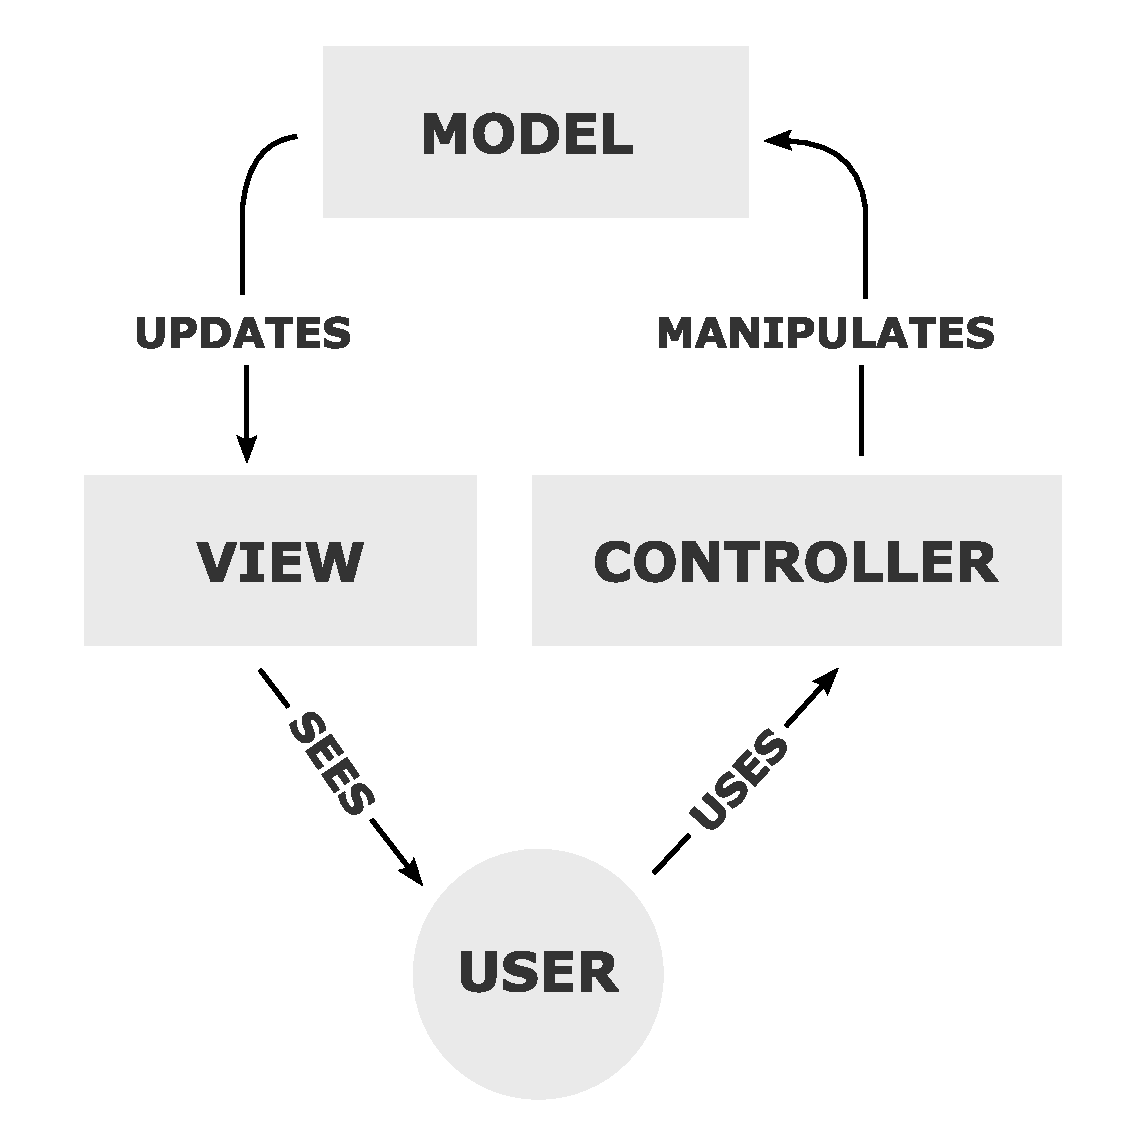
\includegraphics[width=0.75\textwidth]{mvc.pdf}
  \caption{Grundidéen omkring MVC. Fra \url{http://commons.wikimedia.org/wiki/File:MVC-Process.svg} } \label{fig:mvc}
\end{figure}


